% Chapter 2

\chapter{Introduction} % Write in your own chapter title
\label{Chapter2}
\lhead{Chapter 2. \emph{Background and Related Work}}


\section{Single-Layer Networks}

Artificial neurons were introduced as information processing devices more than fifty years ago\citep{mcculloch1943logical}. Following the early work, perceptrons were deployed in layers to do pattern recognition job. A lot of resource was invested in researching capability of learning perceptrons theoretically and experimentally. As shown in Figure 2.1, a perceptron computes a weighted summation of its n inputs and then thresholds the result to give a binary output y. We can treat n input as an vector with n elements, and represent the vector as either class A(for output +1) or class B(for output -1).
\graphicspath{ {./Figures/} }
\begin{figure}
\centering
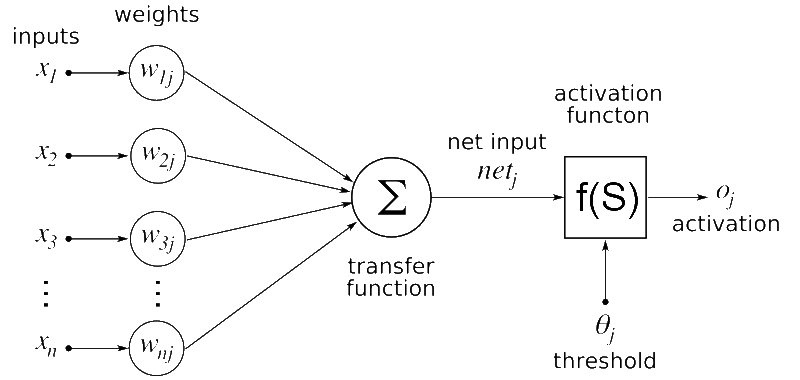
\includegraphics[width=0.8\textwidth]{Figure2-1.png}
\caption{\label{fig:perceptron}Diagram of a perceptron.}
\end{figure}


Each output is updated according to the equation:
\begin{equation}\label{eq:BasicEq}
y_{i} = f(h_{i}) = f\left(\sum_{j}w_{ij}x_{j}\right)
\end{equation}
where $y_{i}$ is the $i$th output, $h_{i}$ is the net input into node $i$, The weight $w_{ij}$ connects the $i$th output and the $j$th input, and $x_{j}$ is the $j$th input. The function $f(h)$ is the activation function and usually makes up the form
\begin{equation}\label{eq:FullEq}
f(h) = sign(h) = 
  \begin{cases}
    -1       & \quad h < 0 \\
    1  & \quad h \geq 0\\
  \end{cases}
\end{equation}
We can also represent \ref{eq:FullEq} in vector notation, as in 
\begin{equation}\label{eq:UsedEq}
y = f(h) = f(\bf w \cdot x)
\end{equation}
where \textbf{w} and \textbf{x} can be regarded as $nx1$ dimensional column vectors, and $n$ is the number of input data.
The term $w \cdot x$ in \ref{eq:UsedEq} constructs a $(n-1)$-dimension hyperplane which passes the origin. The hyperplane can be shifted by adding an parameter to \ref{eq:BasicEq}, for example
\begin{equation}\label{eq:WithBias}
y = f(h) = f(\bf w \cdot x + b)
\end{equation}
We can have the same effect by putting a constant value $1$ and increase the size of $x$ and $w$ by one. The extra weight $w$ with fixed value 1 is called \textit{bias weight}; it is adaptive like other weights and provides flexibility to hyperplane. Then we get:
\begin{equation}\label{eq:finalEq}
y = f(h) = f(\sum_{i=0}^{n}w_{i}x_{i})
\end{equation}
The aim of learning is to find a set of weights $w_{i}$ so that:
\begin{align*}
y = f(\sum_{i=0}^{n}w_{i}x_{i}) = 1  & \quad x \in Class A\\
y = f(\sum_{i=0}^{n}w_{i}x_{i}) = 0  & \quad x \in Class B
\end{align*}


\section{Multi-Layer Networks}

Single-layer networks have some important limitation in terms of the representing range of functions. We are seeking to learn the nonlinearity as the linear discriminant.To improve the representation capability, we can stack layers networks. This is the approach of multilayer neural networks. Multilayer neural networks implement linear discriminants via mapping input data to a nonlinear space. They can use fairly simple algorithms to learn form of the nonlinearity from training data.

In the thesis, we limit multi-layer networks in subset of feedforward networks. As feedforward networks can provide a general mechanism for representing nonlinear functional mapping between a set of input data and a set of labels. The \ref{fig:ffnet} is a feedforward network having two layers of adaptive weights.

\begin{figure}[!htb]
\centering
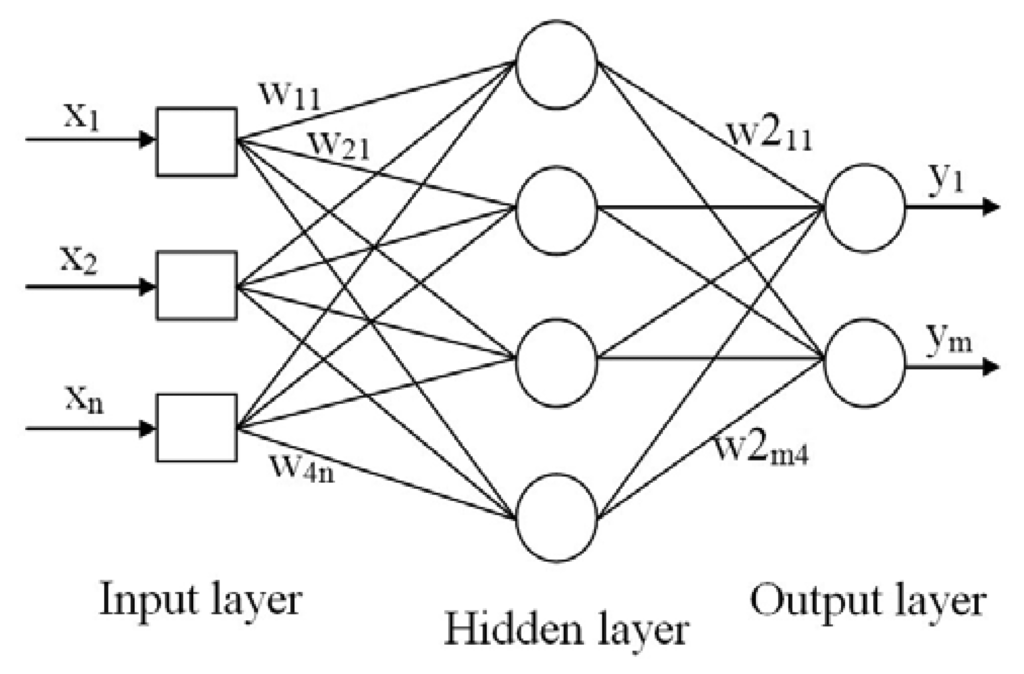
\includegraphics[width=0.8\textwidth]{Figure2-2.png}
\caption{\label{fig:ffnet}Diagram of a feedford neural networks.}
\end{figure}

In the example, the middle column perceptrons act as hidden units. The network has $n$ inputs, $4$ hidden units and $m$ output units. The network diagram represents the function in the form
\begin{equation}\label{eq:ffEq}
y_{m} = \hat{f}\Big(\sum_{j=0}^{m}w_{j4}^{(2)}f\big(\sum_{i=0}^{n}w_{4i}^{(1)}x_{i}\big)\Big)
\end{equation}
In the \ref{eq:ffEq}, outer activation function could be different with the inner one.

There are some choices for activation functions, sigmoid and tanh are related and can provide high capability with continuous input data. Logistic activation function sigmoid can be represented as 
\begin{equation}\label{eq:sigmoid}
f(x) = \frac{1}{1+e^{-x}}
\end{equation}
Its outputs lies in range $(0,1)$. We can do a linear transformation $hat{x}=x/2$ on input data and a linear transformation $hat{y}=2y-1$ on the output. Then we can get an equivalent activation function tanh which can be represented as
\begin{equation}\label{eq:tanh}
f(x) = tanh(x) = \frac{e^{x}-e^{-x}}{e^{x}+e^{-x}}
\end{equation}

The three layer neural network is capable of approximating any function with enough hidden units which means the networks with two layers of weights and sigmoid nonlinearities can provide any accuracy in classification problems. 


\section{Backpropagation}

Multi-layer neural networks can represent mapping from input data to output classes. How to learn a suitable mapping from training dataset? And there is no explicit mapping between output and hidden units. This will be resolved by a popular learning algorithm-backpropagation.

Because networks have differentiable activation functions, the activation of output units can be propagated to hidden units with regard to weights and bias. If we have an error function, we can evaluate derivatives of the error and update the weights to minimize the error function via some optimization methods.

Backpropagation can be applied to find the derivatives of an error function related to the weights and biases in the network via two stages. First, the derivatives of the error functions, for instance sum-of-squares and Jacobian, with respect to the weights must be evaluated. Second, a variety of optimization schemes can be implemented to compute the adjustment of weights based on derivatives. After putting data forward propagation through the network, we can get the output result. It updates weight changes based on grandient descent. Suppose the network has $i$ inputs, $h$ hidden units and $k$ outputs. The update equation can be represented as 
\begin{equation}\label{eq:UpdateWeights}
w(j+1) = w(j) + \Delta w(j)
\end{equation}
where $\Delta w(j)$ defined as 
\begin{equation}\label{eq:DeltaWeights}
\Delta w(j) = -\eta \frac{\partial E}{\partial w}
\end{equation}

For the hidden to output layer weights
\begin{equation}\label{eq:h2oBP}
\Delta w(jk) = -\eta \frac{\partial E}{\partial w_{jk}} = -\eta \delta_{k}y_{j}
\end{equation}
where $$\delta_{k} = \frac{\partial E}{\partial a_{k}} = (y_{k} - t_{k})y_{k}(1 - y_{k})$$

For the hidden layer weights
\begin{equation}\label{eq:hiddenBP}
\Delta w(ij) = -\eta \frac{\partial E}{\partial w_{ij}} = -\eta \delta_{j}y_{i}
\end{equation}
where $$\delta_{j} = \frac{\partial E}{\partial a_{j}} = \displaystyle\sum_{k} \delta_{k}w_{jk}y_{j}(1 - y_{j})$$

The $\delta_{j}$ of a hidden unit is based on the $\delta_{k}$s of output units to which it links. To minimise the error function$E$ with gradient descent, it needs the propagation of errors backwards.

\section{Training protocols}

In supervised learning, we have training dataset which is data with labels. We can use the neural networks to find the output of the training data and adjust the weights to optimal values. There are mainly  three types of training protocols, stochastic, batch and online training. In stochastic training, we randomly choose samples from training dataset and update weights every time depending on output of neural networks. In batch training, we use some samples and pass them through network, then update weights. In online training method, each sample of training dataset is used once and weights are updated each time. We usually call one time of passing all training dataset through neural networks one epoch.

\section{Stochastic Gradient Descent}

Because weights space in neural networks is continuous, training can reach the optimal weights value through optimization algorithms, which means minimizing loss value of function
\begin{equation}\label{eq:LossMin}
L(f_{w}) = \sum L(y, f_{w}(x))
\end{equation}
Gradient descent is a method which starts from a random point, then moves to a nearby point that is downhill repeatly. It converges on a minimum possible loss.

Stochastic gradient descent is a subtype of gradient descent. It only considers a single training point and move to nearby point based on
\begin{equation}\label{eq:SGDUpdate}
w = w - \eta  \Delta L(w) = w - \eta \sum_{i=1}^{n} \Delta L_{i}(w)
\end{equation}
where $\eta$ is the learning rate and $L_{i}(w)$ is the value of the loss function at the $i^{th}$ sample. Although stochastic gradient descent does not guarantee convergence, it is fast.

\section{Convolutional Neural Networks}

Convolutional Neural Networks\citep{lecun1998gradient} are widely applied in image data and they achieved top rank in image classification competetion\citep{krizhevsky2012imagenet}. Convolutional neural networks have three types of layers, convolutional layer, pooling layer and fully connected layer. At the output of the network, a softmax layer is used to do classification job.  Convolutional layer is used to detect invariants in locat receptive fields. Pooling layer is downsampling feature maps. Fully connected layer makes the output of each unit an activation of dot product of all inputs.

\graphicspath{ {./Figures/} }
\begin{figure}[!htb]
\centering
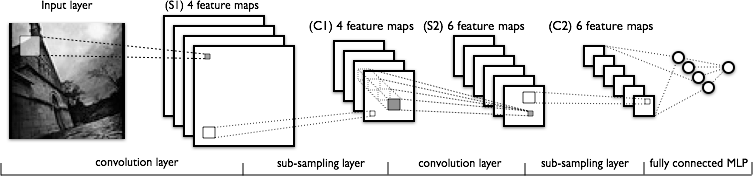
\includegraphics[width=0.8\textwidth]{lenet.png}
\caption{\label{fig:perceptron}Diagram of LeNet.}
\end{figure}

\section{Spatial Pyramid Match}

Spatial pyramid match\citep{lazebnik2006beyond} is used to classify high-level semantic attributes, based on low-level features. The method subdivides a image in several different levels of resolution and counts features falling in each spatial bin. It extends bags of features and derives spatial information from images.
\graphicspath{ {./Figures/} }
\begin{figure}[!htb]
\centering
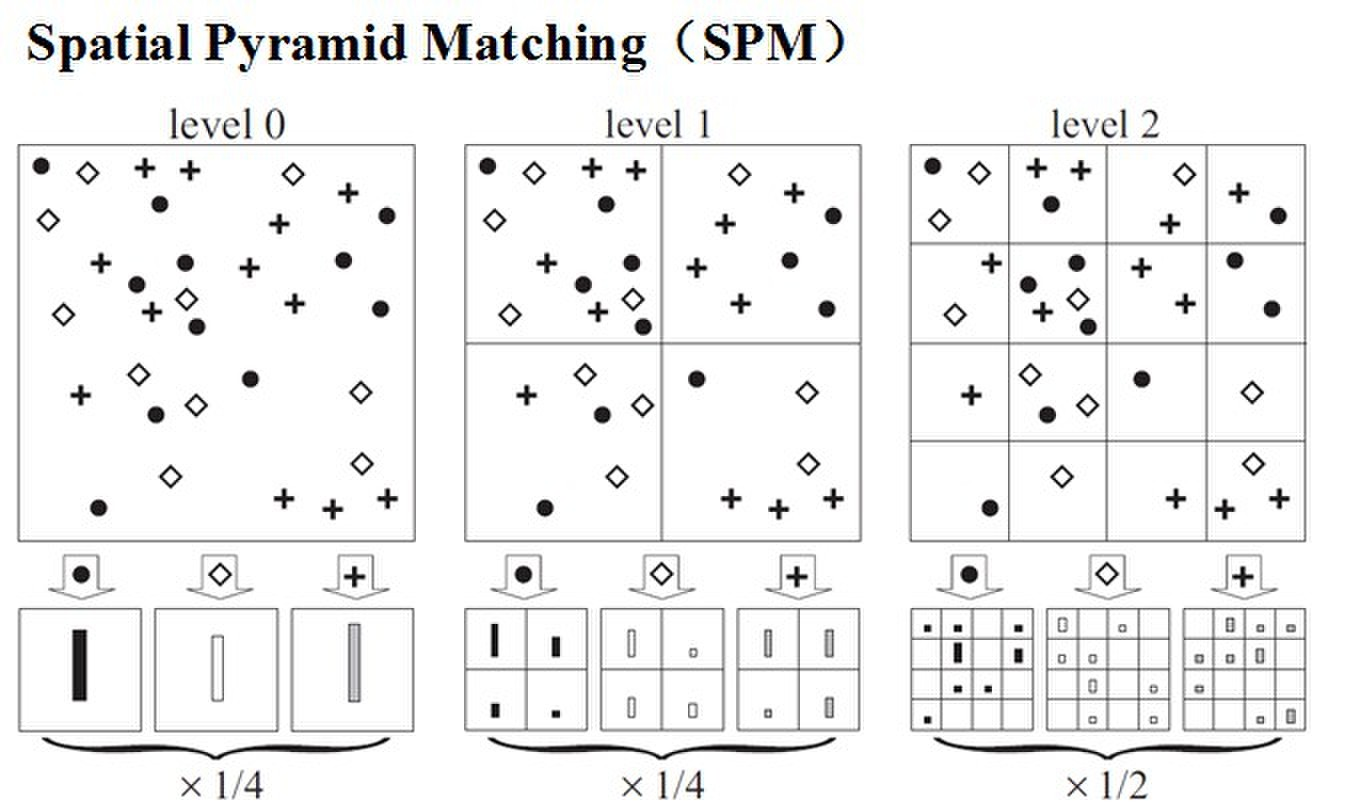
\includegraphics[width=0.8\textwidth]{spm.jpg}
\caption{\label{fig:perceptron}Diagram of Spatial Pyramid Match.}
\end{figure}

\section{Transfer Learning}

In machine learning literature, transfer learning\citep{pan2010survey} focuses on storing knowledge from one domain and applying it to a related problem. It has two benefits. One is saving time to build a model from scratch up. Another is saving effort to collect training data.

A domain with two components, a feature space and a marginal probability distribution, can be represented
\begin{equation}\label{eq:TransLearning}
D = \{ \chi, P(X) \}
\end{equation}
where $\chi$ is feature space and $P(X)$ is the marginal probability distribution. 
\graphicspath{ {./Figures/} }
\begin{figure}[!htb]
\centering
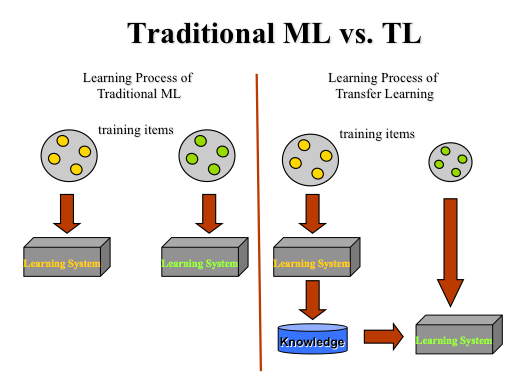
\includegraphics[width=0.8\textwidth]{MLvsTL.png}
\caption{\label{fig:perceptron}Diagram of Transfer Learning.}
\end{figure}
